Machine Learning is since .. Nobel price 2024


\section{Graph Neural Networks}
Graph neural networks are a special Variant of Neural networks that apply to graph shaped data.
In our case the graph is the molecular structure of the system that we want to model. Each atom functions as a node in the graph which contains information about the local density around this atom in form of the coefficients of the basis function that centered on the atom. The Edges of the graph contain information in form of the distance towards the next atom. These distances can be embedded in the edge features of the graph neural network.

\subsection{Messagepassing Neural Network}
Message Passing Neural Networks (MPNNs) operate on graph-structured data G = (V, E), where V is the set of nodes and E is the set of edges. The core of MPNNs is the message passing operation, defined as:

\begin{align}
m_t^(v) &= AGG({M_t(h_t^(v), h_t^(u), e_vu) | u ∈ N(v)})\\
h_(t+1)^(v) &= U_t(h_t^(v), m_t^(v))
\end{align}

where h_t^(v) is the hidden state of node v at time step t, e_vu is the edge feature between nodes v and u, N(v) is the neighborhood of v, M_t is the message function, AGG is an aggregation function (e.g., sum, mean, max), and U_t is the update function. These operations are performed for T time steps to capture higher-order interactions in the graph.

\subsubsection{Embeddings}
The atomic number of every atom is one hot encoded into a vector which length the number of distinct atomtypes in the dataset is. The distance between the atoms Is embedded using besselfunction following the approach of \cite{https://arxiv.org/pdf/2003.03123}. See figure \ref{fig:bessel_embedding}
\begin{align}
    \tilde{e}_{\text{RBF},n}(d) &= \sqrt{\frac{2}{c}}\frac{\sin(\frac{\omega_n }{c})}{d}\hspace{2cm} \omega_n :=(n+1)d\pi\\
    u(d)&= 1-\frac{(p+1)(p+2)}{2}d^p + p(p+2)d^{p+1}-\frac{p(p+1)}{2}d^{p+2}
\end{align}
Where we choose p = 1 and c = 6, as most of the bonds in our dataset are shorter than 6 Angstrom as can be seen in figure \ref{fig:bond_length}. The distance embedding is then multiplied with the one hot encoded atomic number of the atom to get the final edge feature.

\begin{figure}
    \centering
    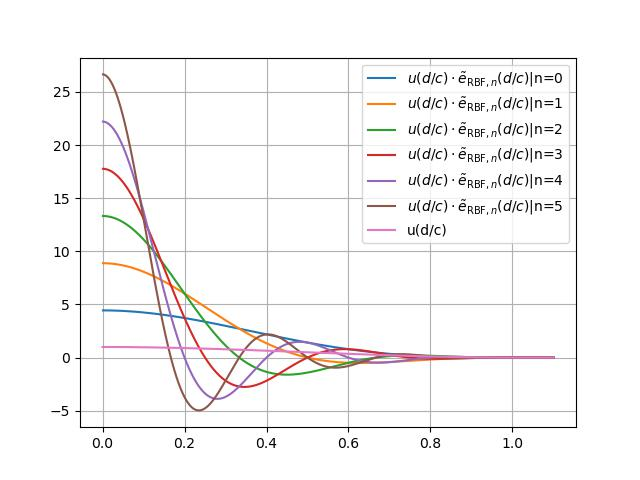
\includegraphics[width=0.8\textwidth]{chapters/foundations/images_foundation/bessel_embedding}
    \caption{The initial basis function used for the distance embedding in the graph neural network.}
    \label{fig:bessel_embedding}
\end{figure}
\begin{figure}
    \centering
    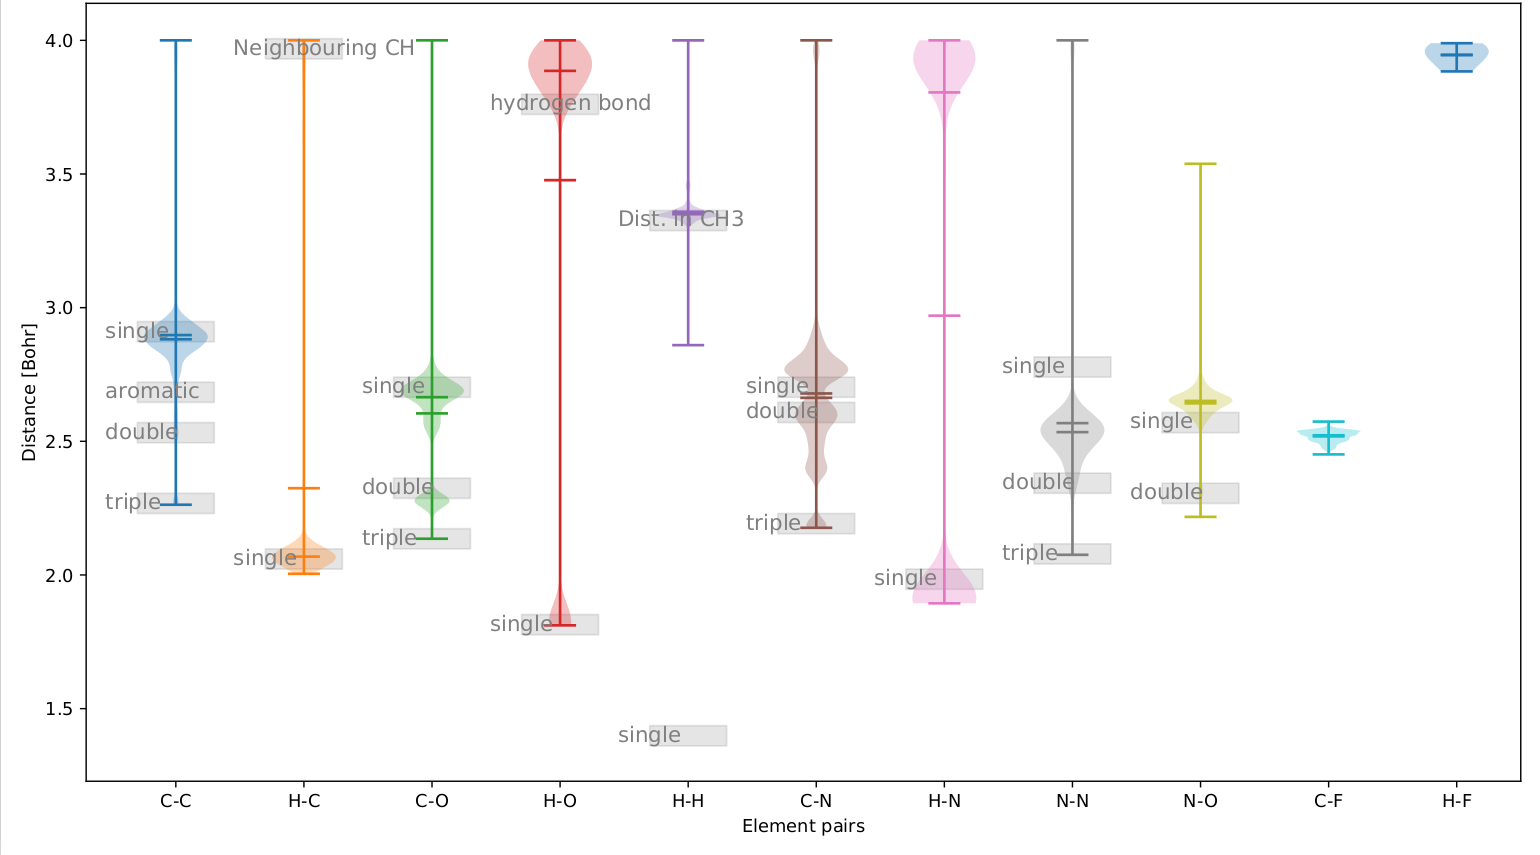
\includegraphics[width=0.8\textwidth]{chapters/foundations/images_foundation/bondlength}
    \caption{The average Bondlength appearing in QM9(Credit Tobias)}
    \label{fig:bond_length}
\end{figure}
For the final embedding of the edge features the one hot encoded atomic number of the incomming and outcomming atom is concatenated with the distance embedding. This is then passed through a short MLP\cite{mlp} with scip connection:
%\begin{align}
%        h_i:= \text{HOTONE(z_i)}\in R^{n_z}\\
%        e_{\text{edge embedding},i,j}^{(0)} = \sigma((h_i||h_j||\text{emb_{ij}})W_{\text{edge}}+b_{\text{edge}})\\
%    e_{\text{edge embedding},i,j}^{(1)} &= u(d_{i,j})(x_{\text{edge embedding}}^{(0)} + \text{MLP}(x_{\text{edge embedding}}^{(0)}))
%\end{align}
These edge features are then aggregated into node features using an aggregation function. The Node features are then futher processed.
\begin{align}
    n_{node_{features}}_i^{(0)} = \text{AGG}(e_{\text{edge embedding},i,j}^{(1)})_i + h_{i}W_{\text{node}}+b_{\text{node}}\\
    n_{node_{features}}_i^{(l+1)} = text{BathNorm}(\n_{node_{features}}_i^{(l)}+ \text{MLP}(n_{node_{features}}_i^{(l)}))
\end{align}
Then iterativly new edge messages are contructed from these node features and again aggregated to node features:
\begin{align}
    e_{\text{edge embedding},i,j}^{(l+1)} = \text{MLP}(n_{node_{features}}_i^{(l)}||n_{node_{features}}_j^{(l)}||e_{\text{edge embedding}}_i,j^{(l)})\\
    n_{node_{features}}_i^{(l+1)} = \text{AGG}(e_{\text{edge embedding},i,j}^{(l+1)})_i + n_{node_{features}}_i^{(l)}
\end{align}
\subsection{Graphformer}
The architecture for the much more expressive model used for OFDFT is the Graphformer. The Graphformer is a transformer like architecture that operates on graph structured data, in this case a complete graph but takes into account the distances between different nodes in its attention module. \cite{Graphformer}.
We also intotroduce a Atomic reference module as it was done in Mofdft\cite{zhang_m-ofdft_2023}.
